\documentclass[12pt]{article}

\usepackage{listings}
\usepackage{xcolor}

\lstdefinestyle{sharpc}{language=[Sharp]C, frame=lr, rulecolor=\color{blue!80!black}}

\definecolor{mGreen}{rgb}{0,0.6,0}
\definecolor{mGray}{rgb}{0.5,0.5,0.5}
\definecolor{mPurple}{rgb}{0.58,0,0.82}
\definecolor{backgroundColour}{rgb}{0.95,0.95,0.92}

\lstdefinestyle{CStyle}{
    backgroundcolor=\color{backgroundColour},   
    commentstyle=\color{mGreen},
    keywordstyle=\color{magenta},
    numberstyle=\tiny\color{mGray},
    stringstyle=\color{mPurple},
    basicstyle=\footnotesize,
    breakatwhitespace=false,         
    breaklines=true,                 
    captionpos=b,                    
    keepspaces=true,                 
    numbers=left,                    
    numbersep=5pt,                  
    showspaces=false,                
    showstringspaces=false,
    showtabs=false,                  
    tabsize=2,
    language=C
}



\usepackage{fullpage} %permite folosirea intregii pagini
\usepackage{tocloft} %pachet pentru table of contents
\usepackage{float} %pentru a forta img la coordonate specifice
\usepackage{graphicx} %pentru imagini
\usepackage{hyperref} %folosit pentru referinte in toc
\hypersetup{ %setup referinte toc, se fac automat, trebuie
    colorlinks, %compilat de doua ori
    citecolor=black,
    filecolor=black,
    linkcolor=black,
    urlcolor=black
}

\large
\title{Proiect 2 - Documentatie \\ 
Minisistem pentru irigat plante}
\author{Chisalescu Bogdan si Floricel Antonio - Stefan \\
Grupa 432A \\ \\ Coordonator stiintific: S.l. dr. ing. Valentin Stoica}
\date{}

\begin{document}
\large
\maketitle
\newpage


%Schimba numele pentru tableofcontents
\renewcommand*\contentsname{Cuprins}
%Adauga ... in toc
\renewcommand{\cftsecleader}{\cftdotfill{\cftdotsep}}


\tableofcontents
\newpage


\section{Cerinta de proiectare}
\hspace{8 mm} Implementarea unui minisistem pentru irigat plante folosind microcontrolerul Atmel AVR ATmega 164A. Realizarea fizica trebuie efectuata pe o placa de cablaj imprimat cu componente SMD furnizata de catre facultate, insa datorita conditiilor epidemiologice si masurilor luate de Conducerile ETTI si UPB aceasta modalitate de realizare nu a fost posibila; masurile de distantare sociala si invatamant in regim "online" au facut impractic accesul la aparatura necesara, astfel am decis realizarea proiectului pe placi de prototipare si cu componente THT. Realizarea in formatul SMD + placa de circuit imprimat s-ar fi putut realiza de catre un singur membru al echipei insa in acest mod contributia asupra proiectului ar fi fost sever dezechilibrata. Intelegem ca in urma acestei decizi se pierd anumite avantaje precum stabilitatea cu temperatura, zgomotul redus, costul redus, etc.
\\

\section{Solutia de implementare propusa}
\hspace{8 mm} Pentru a implementa minisistemul de irigat plante  vom avea nevoie de doua clase principale de componente: senzori si actuatori. Actiunea de a iriga plantele consta in transferul unei cantitati de apa dintr-un rezervor catre plante. Pentru a decide momentul irigarii si a o efectua este nevoie de prelucrarea marimilor fizice implicate si anume umiditatea solului si disponibilitatea apei din rezervor reprezentata prin nivel (inaltimea coloanei de apa). Pentru a extrage si cuantifica aceste marimi vom folosi un senzor de umiditate a solului si unul de nivel. Pentru transportul apei de la rezervor la plante vom folosi ca actuator o minipompa de apa. Pentru a facilita interactiunea cu sistemul al unui posibil utilizator vom dezvolta o aplicatie desktop ce va asigura transmisia de date de configurare plus o serie de informatii despre starea sistemului in timp real.
\\

\section{Schema bloc a sistemului}
\hspace{8 mm} Schema bloc a sistemului reprezinta arhitectura generala si descrie modul conceptual de interconectare a componentelor. Se poate observa o comunicatie unilaterala intre blocuri precum senzorii si microcontroler si o comunicatie bilaterala intre microcontroler si aplicatia utilizatorului, acestea semnificand sensul de transmitere al informatiei.
\\

\begin{figure}[H]
\centering
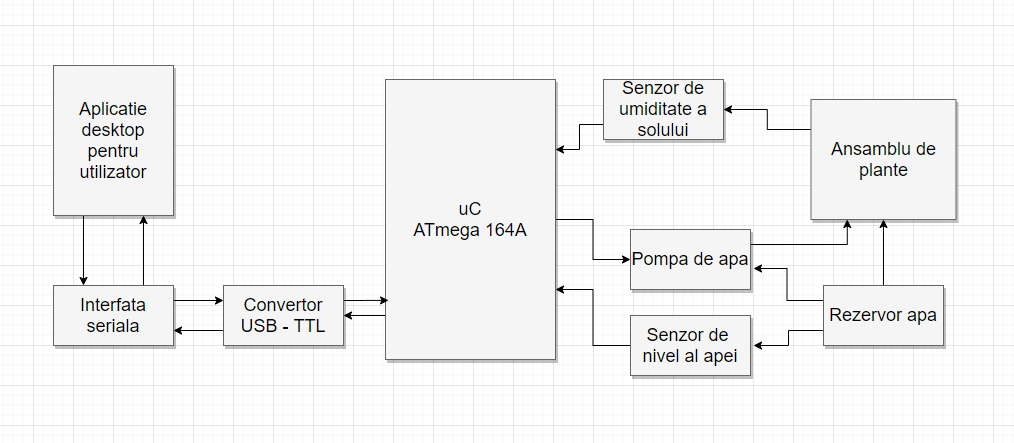
\includegraphics[width=\textwidth]{Pictures/schemaBloc.png}
\caption{Schema bloc a minisistemului de irigat plante}
\end{figure}

\vspace{4 mm}

\section{Incarcarea codului pe microcontroler}

\hspace{8 mm} Microcontrolerul dispune de mai multe modalitati prin care poate fi programat. Cele care sunt de interes sunt programarea folosind un programator dedicat si programarea folosind un bootloader. Utilizarea programatorului dedicat este simpla intrucat este necesara doar conexiunea sa catre PC prin portul USB si realizarea conxiunilor catre pinii dedicati ai microcontrolerului. Utilizarea bootloaderului presupune intai scrierea acestuia intr-o memorie nonvolatila, spatiul rezervat acestuia fiind in adresele superioare are memoriei Flash de program. Dupa incarcarea bootloaderului nu mai este nevoie de programatorul dedicat deoarece in procesul de programare al microcontrolerului bootloaderul preia controlul folosind ce interfata seriala are la dispozitie, incarca aplicatia ce va rula pe microcontroler in memroia de program si ulterior ii cedeaza acesteia controlul executiei. In aceasta lucrare am optat pentru incarcarea codului cu un programator dedicat deoarece ne confera mai multe functionalitati. Am ales pentru elaborarea codului mediul de dezvoltare Atmel Studio 7 acesta fiind creat special pentru programarea microcontrolerelor fabricate de Atmel. Cu ajutorul Atmel Studio si compilatorului GCC vom crea un fisier cu extensia .hex ce va fi incarcat pe microcontroler de catre softul "avrdude" folosind comanda "avrdude -c usbasp -p m164p -U flash:w:\$(ProjectDir)Debug\ \$(TargetName).hex:i". Deoarece avrdude nu ofera suport pentru modelul ATmega 164A, am modificat in fisierul de configurare al avrdude semnatura dispozitivului alegand cel mai apropiat dispozitiv ca arhitectura de ATmega 164A, acesta fiind ATmega 164P.

\begin{figure}[H]
\centering
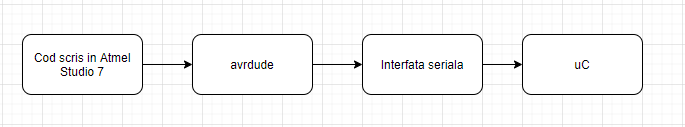
\includegraphics[width=\textwidth]{Pictures/avrdudePath.png}
\caption{Modul in care se incarca codul pe uC}
\end{figure}

\vspace{4 mm}

\section{Cuplarea unui oscilator extern}
\hspace{8 mm} Atmega 164A pune la dispozitie o multitudine de optiuni cand vine vorba de alegerea sursei pentru ceasul intern; acesta vine echipat cu un oscilator RC intern calibrat la frecventa de 8 MHz, iar pentru ceasul de sistem aceasta frecventa este impartita la 8, de unde rezulta 1 MHz, astfel in mod implicit microcontrolerul ruleaza la o frecventa de ceas de 1 MHz. Deoarece aceasta frecventa de 1 MHz este in anumite situatii un factor limitator de performanta vom cupla un oscilator extern cu cristal de quartz de 20 MHz. Pentru a determina microcontrolerul sa foloseasca acest oscilator ca sursa pentru ceasul de sistem este nevoie sa fie modificati bitii fuse. Bitii fuse sunt localizati intr-o zona rezervata din memoria EEPROM iar modificarea acestora se poate face numai cu un programator dedicat deoarece bootloaderul nu poate accesa acel sector al memoriei. Bitii fuse sunt o serie de biti ce ajuta la configurarea microcontrolerului, aceastia formeaza impreuna 3 bytes: High Fuse Byte, Low Fuse Byte si Extended Fuse Byte, pentru fiecare bit "1" inseamna programat iar "0" inseamna neprogramat. Pentru a fi siguri ca am programat corect acesti biti am folosit resursa https://www.engbedded.com/fusecalc/, unde am ales tipul de oscilator in conformitate cu foaia de catalog a microcontrolerului adica Full Swing Crystal Oscilator cu timp de pornire cat mai mare ca sa asigure o durata suficienta stabilizarii oscilatiilor si am dezactivat optiunea ce imparte ceasul la 8. Modificarea bitilor fuse a fost efectuata cu programul avrdude folosind comanda "avrdude -c usbasp -p m164p -U lfuse:w:0xe7:m -U hfuse:w:0x99:m". Pentru a ne asigura ca microcontrolerul foloseste intradevar frecventa de 20 MHz, am definit in cod frecventa ceasului la un 1 MHz si am tinut aprins un LED timp de 2 secunde. In acest caz frecventa ceasului intern fiind de 1 MHz, LED-ul a stat aprins pentru 2 secunde, exact cat a fost programat(..insert link here...). Am cuplat apoi oscilatorul si am rulat acelasi program, in acest caz LED-ul nu mai sta aprins timp de 2 secunde, ci mult mai putin(...insert linke here...). In cod am definit frecventa de 1 MHz iar microcontrolerul presupune ca aceasta este frecventa ceasului intern si calculeaza in functie de ea timpul pentru care tine LED-ul aprins, iar apoi pentru a-l tine aprins utlizeaza ceasul intern, de aceea chiar daca calculul s-a facut pentru o frecventa de 1 MHz, LED-ul nu va sta aprins pentru 2 secunde deoarece frecventa ceasului este mult mai mare, in acest caz 20 MHz iar timpul in care sta LED-ul aprins este de 0.1 secunde. In urma acestui test putem spune cu exactitate ca microcontrolerul seteaza ceasul intern dupa oscilatorul cuplat.

\begin{figure}[H]
\centering
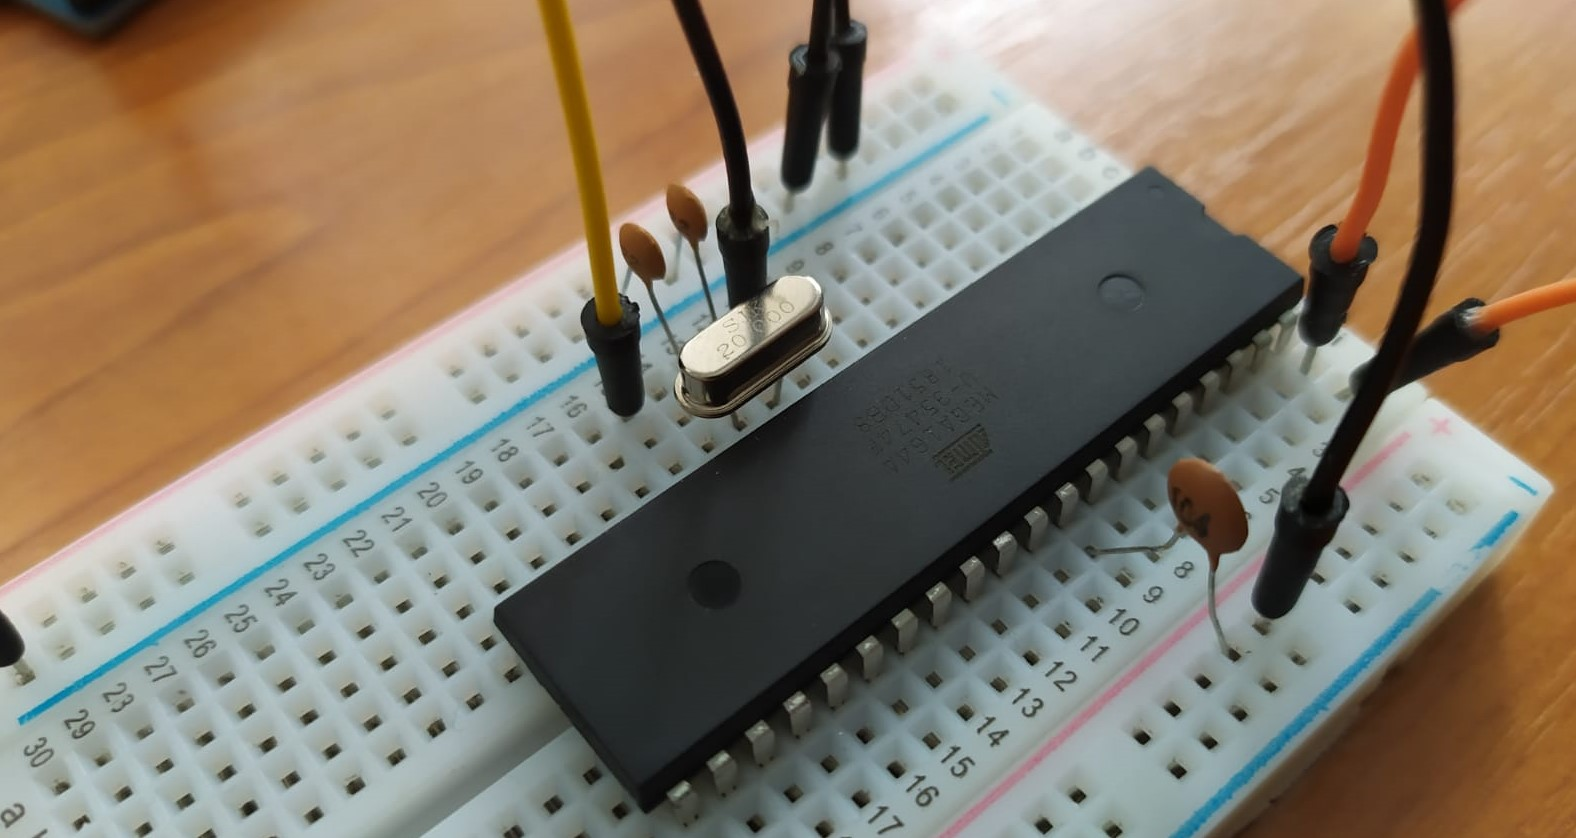
\includegraphics[width=\textwidth]{Pictures/osc.jpeg}
\caption{Oscilatorul cuplat la uC conectat la pinii XTAL1 si XTAL2 cu 2 condensatoare de 22 pF, valori extrase din foaia de catalog.}
\end{figure}

\begin{figure}[H]
\centering
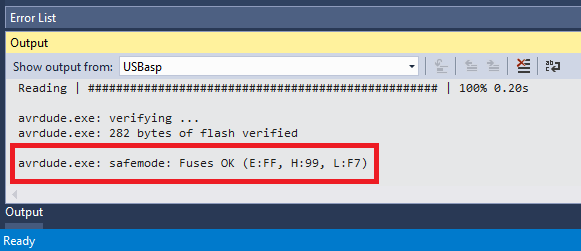
\includegraphics[width=\textwidth]{Pictures/fuse.png}
\caption{Programarea bitilor fuse cu avrdude USB ASP}
\end{figure}

\newpage


\section{Comunicatia seriala}
\hspace{8 mm} Microcontrolerul este capabil de a comunica cu alte dispozitive, aceasta comunicatie asigurandu-se printr-o multitudine de protocoale si interfete, insa ptrintre acestea nu se afla si USB; de aceea pentru a realiza comunicatia intre uC si PC prin intermediul portului USB este nevoie de un convertor USB-TTL. Rolul acestuia este de a adapta interfata folosita de microcontroler pentru comunicatie la cea folosita de PC pentru a se putea efectua schimbul de informatii. Pe tot parcursul desfasurarii proiectului, din cauza lipsei stocului nu am putut face rost de un convertor USB-TTL dedicat, insa am avut la dispozitie o placa de dezvoltare Arduino ce are integrat un astfel de convertor si poate fi configurata sa functioneze si cu alte dispozitive in afara de uC sau integrat. Legand pinul RESET la GND pe placa de dezvoltare Arduino putem suspenda microcontrolerul integrat al placii si folosi convertorul USB-TTL pentru a comunica cu alte dispozitive prin intermediul pinilor RX si TX. Optional, folosind aceasta placa de dezvoltare se poate asigura alimentarea microcontrolerului.

\begin{figure}[H]
\centering
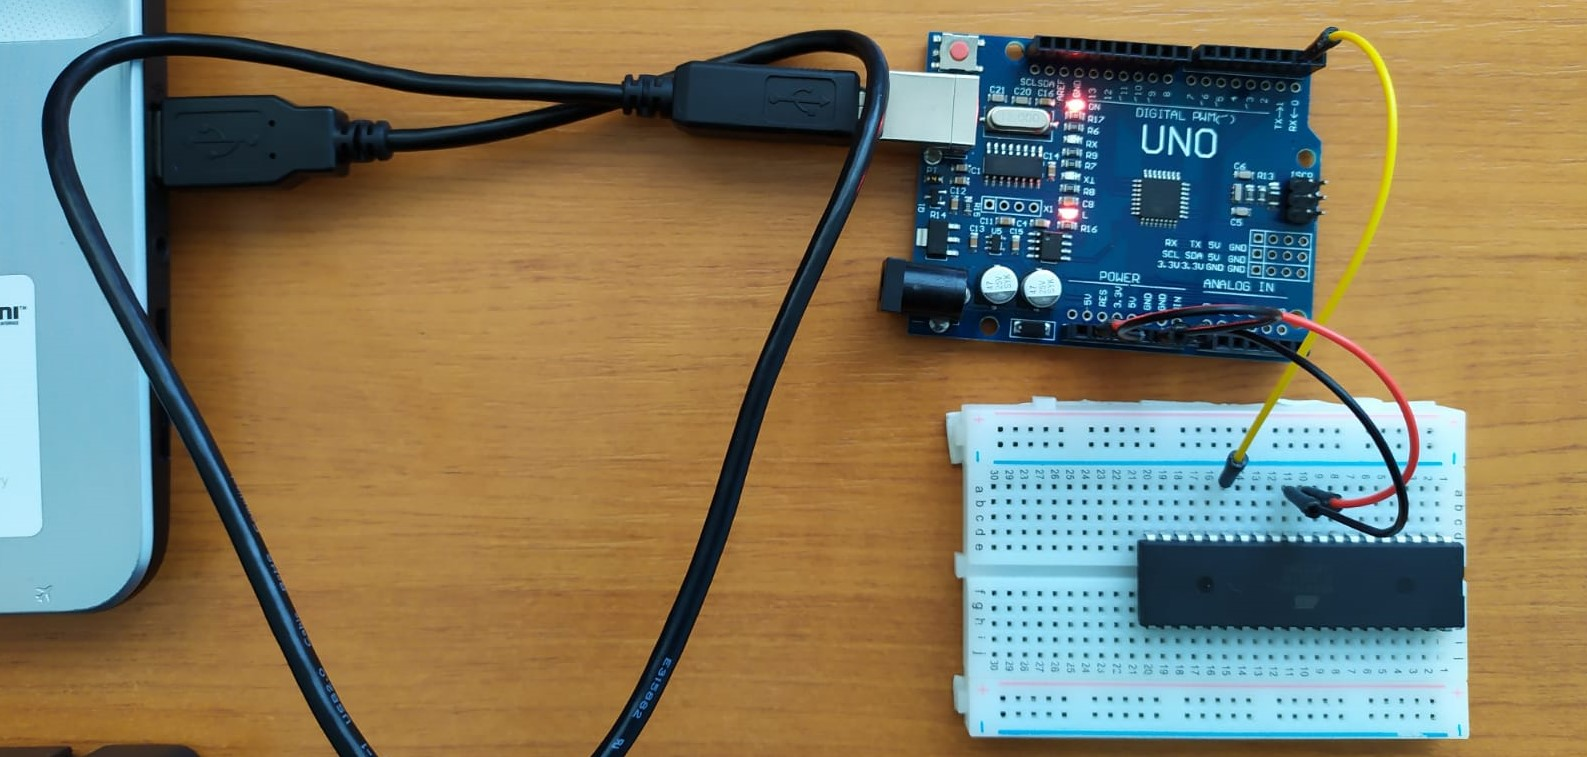
\includegraphics[width=\textwidth]{Pictures/convertor.jpeg}
\caption{Placa de dezvoltare Arduino folosita pe post de convertor USB-TTL}
\end{figure}

\vspace{4 mm}

\hspace{8 mm} ATmega 164A dispune de urmatorele moduri de comunicatie seriala: SPI, USART, USART in modul SPI si TWI. Din cauza familiaritatii, usurintei de implementare si simplitatii am ales sa folosim interfata USART, iar din cele doua prezente in functionalitatea microcontrolerului USART0 si USART1 vom folosi USART0. Pentru o mai mare flexibilitate am ales sa folosim pentru transmiterea si receptionarea datelor modul asincron de lucru, deci se impune setarea unei rate de baud; aceasta este calculata folosind frecventa interna a ceasului si continutul registrului UBBRn. Practic pentru a seta rata de baud este necesara scrierea unei valori in registrul UBBRn, aceasta valoare este deci calculata dupa formula $UBBRn = \frac{f_{OSC}}{16BAUD}-1$. Datele vor fi transmise in aceasta comunicatie in formate. Un format de date suporta 1 bit de start, 5 pana la 9 biti de date, 1 bit de paritate si unul sau doi biti de stop. Linia de comunicatie ramane la nivelul logic de 1 in starea de asteptare dupa care schimbarea nivelului catre nivelul de 0 logic semnifica aparitia bitului de start, apoi sunt transmisi cei 5 pana la 9 biti de date, bitul de paritate optional si bitii de stop, dupa care linia ramane din nou in asteptare, stare corespunzatoare nivelului de 1 logic pana la urmatoarea transmisie a altui format de date. Deoarece dimensiunea datelor cu care lucram se poate exprima in functie de numarul de octeti pe care il ocupa in memorie, cea mai convenabila alegere este cea de 8 biti de date. In aceasta comunicatie sursele de interferenta sunt minime, astfel ca am deci transmisia fara bitul de paritate iar pentru simplitate ne vom rezuma la un bit de stop.


\begin{figure}[H]
\centering
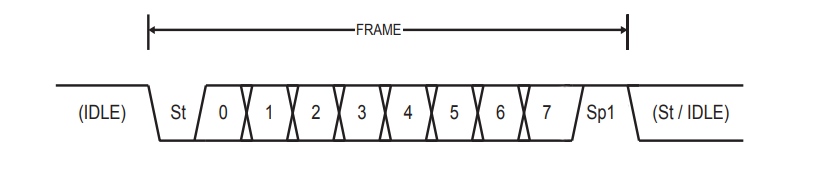
\includegraphics[width=\textwidth]{Pictures/frame.png}
\caption{Formatul de date ales in cadrul acestui proiect}
\end{figure}

\vspace{4 mm}

\hspace{8 mm} Setarea tuturor parametrilor dar si controlul transmisiei si receptiei se efectueaza cu ajutorul a 3 registre speciale de stare si control: UCSR0A, UCSR0B si UCSR0C. Deoarece timpul nu este o variabila critica in acest proiect am ales o rata de baud de 9600 simboluri/s. Pentru a activa transmisia si receptia se seteaza bitii TXEN0 si respectiv RXEN0 din registrul UCSR0B. Arhitectura AVR a acestui microcontroler ne pune la dispozitie registrul UDR0 pentru schimbul de informatii, registru de deplasare pe 8 biti. In momentul in care acest registru este scris si daca transmisia este activata se va incepe transmiterea lui pe interfata seriala, iar daca receptia este activata, orice date receptionate se vor gasi in acest registru. Desi denumirea este comuna atat pentru receptie cat si pentru transmisie, modul in care este folosit (daca se scrie sau se citeste) determina care registru este adresat (existand astfel 2 registre cu numele de UDR0), USART facilitand o comunicatie full duplex (se poate transmite si receptiona independent).
\vspace{4 mm}

\section{Etalonarea senzorilor}
\hspace{8 mm} De obicei orice componenta electronica activa sau de o compelxitate ridicata este livrata impreuna cu o foaie de catalog de la producator care descrie in detaliu functionarea acesteia. Din cauza bugetului redus am achizitionat senzori ce nu dispun de foi de catalog, ci numai de o serie de parametrii listati de distribuitor. Chiar daca majoritatea senzorilor au o caracteristica ideala liniara am decis ca este necesara etalonarea pentru a garanta functionarea acestor in anumite limite. Ambii senzori, atat cel de nivel cat si cel de umiditate a solului ar trebui ideal sa aiba caracteristici liniare. Senzorii au o marime de intrare reprezentata de marimea fizica ce trebuie masurata si o marime de iesire, pentru ambii senzori reprezentata de o tensiune electrica ce va trebui citita. Pentru a etalona senzorii vom privi ambele marimi ca doua variabile aleatoare, vom prelua date empirice si vom folosi metode statistice pentru a estima parametrii de interes. Vom nota astfel cu $X$ marimea de intrare si cu $Y$ marimea de iesire si vom incerca estimarea liniara a variabilei $Y$ cu ajutorul variabilei $X$ determinand o functie de forma $\hat{Y} = \varphi(X)$. Pentru a determina aceasta functie vom utiliza metoda celor mai mici patrate prin care ne dorim ca $M[(Y-\varphi(X))^2] = min$. In cazul nostru cea mai buna estimare este una de tip liniar si neomogen astfel ca $\hat{Y}$ va fi de forma $\hat{Y} = aX + b, \\ a,b \in \Re$. Microcontrolerul va citi variabila $Y$ si va incerca sa estimeze valoarea lui $X$ de aceea dupa determinarea dependentei intre $X$ si $Y$ vom determina inversa functiei adica $\varphi^{-1}$. Pentru ambii senzori am ales sa prelucram datele folosind mediul Matlab si am determinat caracteristica trasand un polinom de gradul unu ce minimizeaza media patratului erorii $\varepsilon = Y-\varphi(X)$. In Matlab ne-au fost returnati coeficientii $a,b \in \Re$ ai acestui polinom.

\subsection{Senzorul de nivel al apei}

$X$ = nivelul apei [mm]\\
$Y$ = tensiunea de iesire [V] \\
Pentru acest senzor am efectuat 3 masuratori independente, 2 cu senzorul alimentat la 5V cu Vcc mediu de 4.7857V si una la 3V cu Vcc mediu de 3.24V, pentru ultima masuratoare senzorul a prezentat o caracteristica puternic neliniara si nu a fost inclusa in calcule, in acelasi timp ne poate sugera ca functionarea senzorului este mai stabila pentru alimentare la 5V. Pentru a determina valorile coeficientilor am conclus ca media primelor doua masuratori este mai apropiata de valoarea reala. \\
Din datele masurate am putut extrage $a = 0.02795, b = 2.044 \Rightarrow \hat{Y} \approx 0.03X + 2$, de unde $\varphi^{-1}(x) = \frac{100x-200}{3}$, deci am obtinut functia ce face legatura intre tensiunea citita si nivelul apei din rezervor. 

\begin{figure}[H]
\centering
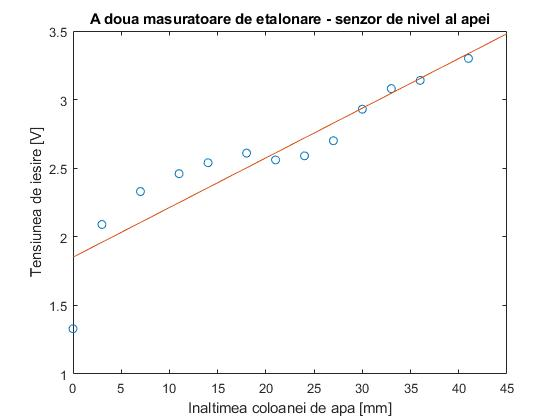
\includegraphics[width=0.76\textwidth]{Pictures/nivelmas.jpg}
\caption{Determinarea caracteristicii senzorului de nivel}
\end{figure}

\newpage

\begin{figure}[H]
\centering
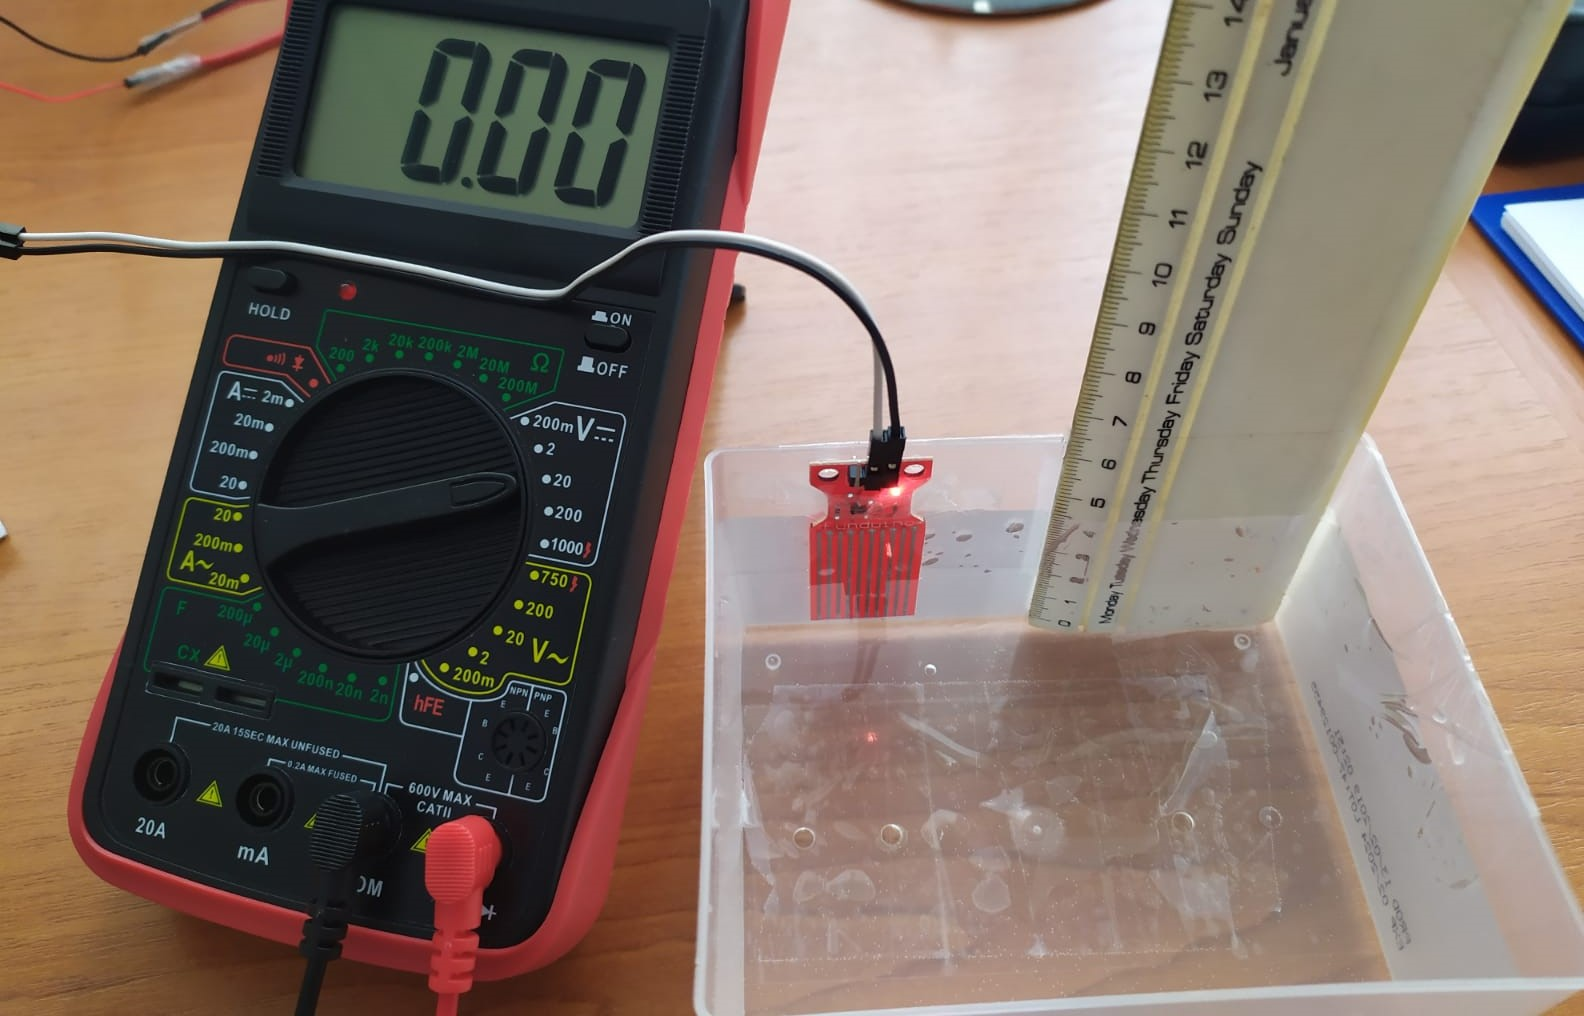
\includegraphics[width=\textwidth]{Pictures/nivelemp.jpeg}
\caption{Masurarea empirica a marimii de iesire pentru senzorul de nivel}
\end{figure}

\begin{figure}[H]
\centering
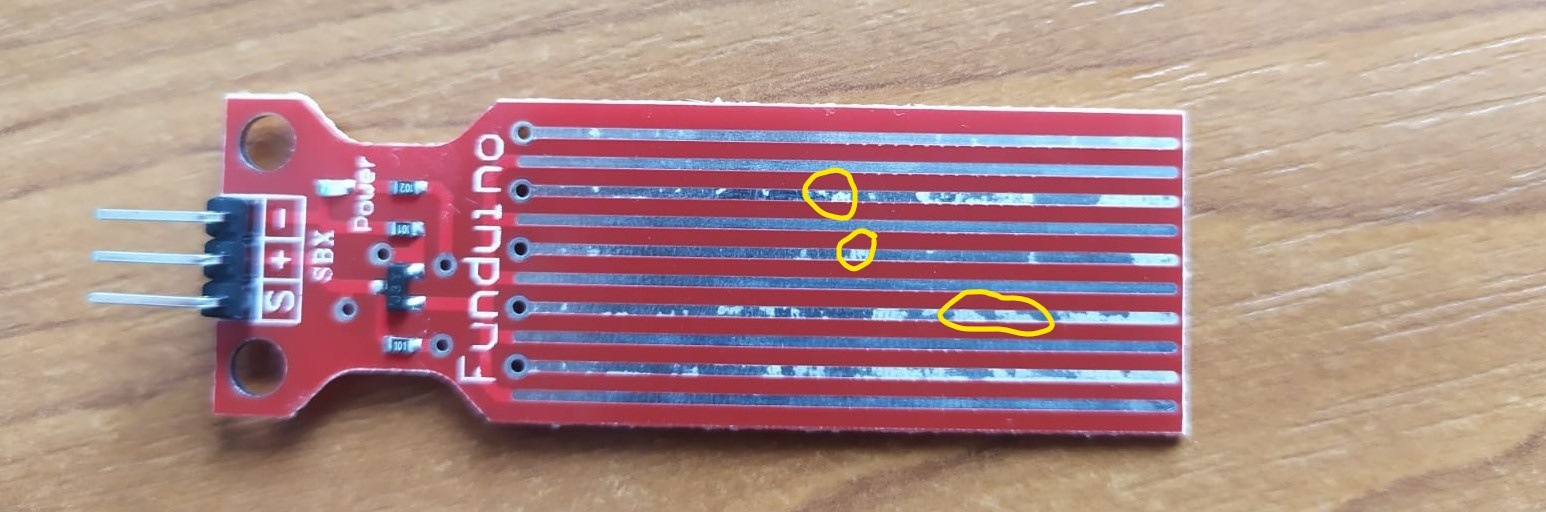
\includegraphics[width=\textwidth]{Pictures/coroziune.jpg}
\caption{Coroziunea aparuta pe suprafata senzorului}
\end{figure}

Pentru ca sezorii achizitionati sunt relativ ieftini acestia nu sunt calitativi, se poate observa o consecinta a acestui fapt prin aparitia pe suprafata senzorului a unui tip de coroziune concentrata in pete. \textcolor{red}{In timp, coroziunea poate afecta performantele senzorului.}

\newpage

\subsection{Senzorul de umiditate a solului}

$X$ = umiditatea solului [\%] \\
$Y$ = tensiunea de iesire [V] \\
Am notat greutatea solului umed = gsum si greutatea solului uscat = gsu, astfel putem calcula umiditatea solului exprimata in procente dupa formula $umiditatea = \frac{gsum - gsu}{gsu} \cdot 100$ [\%]\\
Pentru etalonarea senzorului de umiditate am ales o mostra de sol cu greutatea aproximativa de 100 g. Deoarece nu am avut acces la instrumente de precizie aceasta masuratoare este grosiera, ca atare si aproximarea caracteristicii senzorului va fi una grosiera. \\
Pentru acest senzor am efectuat 3 masuratori insa de data aceasta valorile au fost preluate una dupa cealalta, ceea ce nu ne mai da posibilitatea de a spune ca masuratorile sunt independente, pentru calculul parametrilor am considerat o singura masuratoare unde am mediat fiecare valoare. \\
Din datele masurate am putut extrage $a = -0.042, b = 4.7981 \Rightarrow \hat{Y} \approx -0.04X + 4.8$, de unde $\varphi^{-1}(x) = -5(5x-24)$, deci am obtinut functia ce face legatura intre tensiunea citita si umiditatea solului.

\begin{figure}[H]
\centering
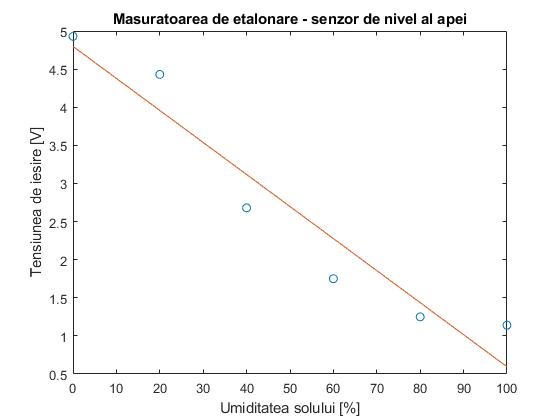
\includegraphics[width=0.76\textwidth]{Pictures/umidmas.jpg}
\caption{Determinarea carcateristicii senzorului de umiditate}
\end{figure}

\newpage

\begin{figure}[H]
\centering
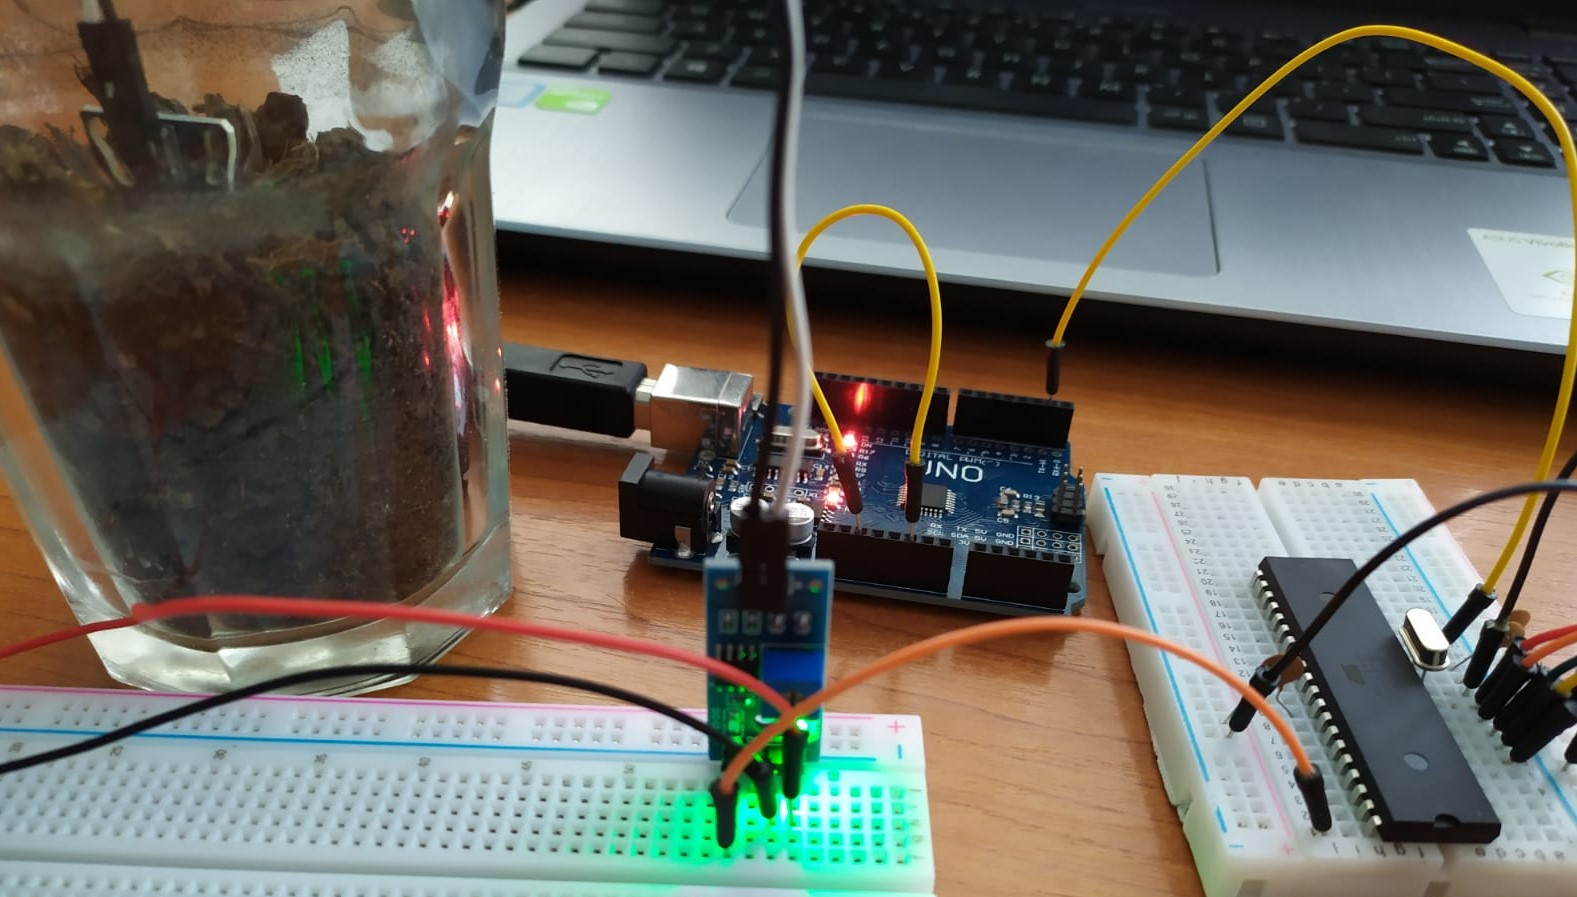
\includegraphics[width=\textwidth]{Pictures/umidemp.jpeg}
\caption{Masurarea empirica a marimii de iesire pentru senzorul de umiditate a solului}
\end{figure}

S-a incercat in paralel si masurarea cu ajutorul microcontrolerului, insa rezultatele furnizate de acesta erau inconsistente si de o deviatie mare fata de valorile date de multimetru, astfel ca nu s-au putut extrage informatii din aceasta masuratoare.


\section{Actuatorul}
\hspace{8 mm} Ca actuator pentru a extrage apa din rezervor si a o transporta catre ansamblul de plante am ales o minipompa de apa submersibila. De asemenea si in cazul acesteia din cauza bugetului am achizitionat o pompa ce nu a venit cu o foaie de catalog ci cu o serie de specificatii din partea distribuitorului. Din pacate pompa a ajuns nefunctionala, insa am reusit sa gasim problema si sa o reparam. Minipompa de apa consta dintr-un motor DC si un ansamblu mecanic format dintr-o paleta si o incapere cu 2 orificii, unul prin care apa intra in incapere si unul prin care iese directionata de paleta, ce este la randul sau pusa in miscare de rotatie de catre motor. Problema pentru pompa noastra a fost ca paleta se afla mult prea aproape de corp ceea ce determina o forta de frecare mult prea mare pentru a fi dezvoltata de motor, si in acest mod chair daca era alimentata, pompa nu functiona. Solutia a constat in deplasarea paletei pe axul ce o conecteaza la motor astfel incat sa se reduca frecarea cu corpul pompei. In urma acestei actiuni am reusit sa facem pompa functionala, insa parametrii sai s-au schimbat. Debitul s-a redus de la 1.2-1.4 L/min la aproximativ 0.43 L/min iar consumul sau de curent este usor crescut de la 250-270 mA la aproximativ 300 mA.


\begin{figure}[H]
\centering
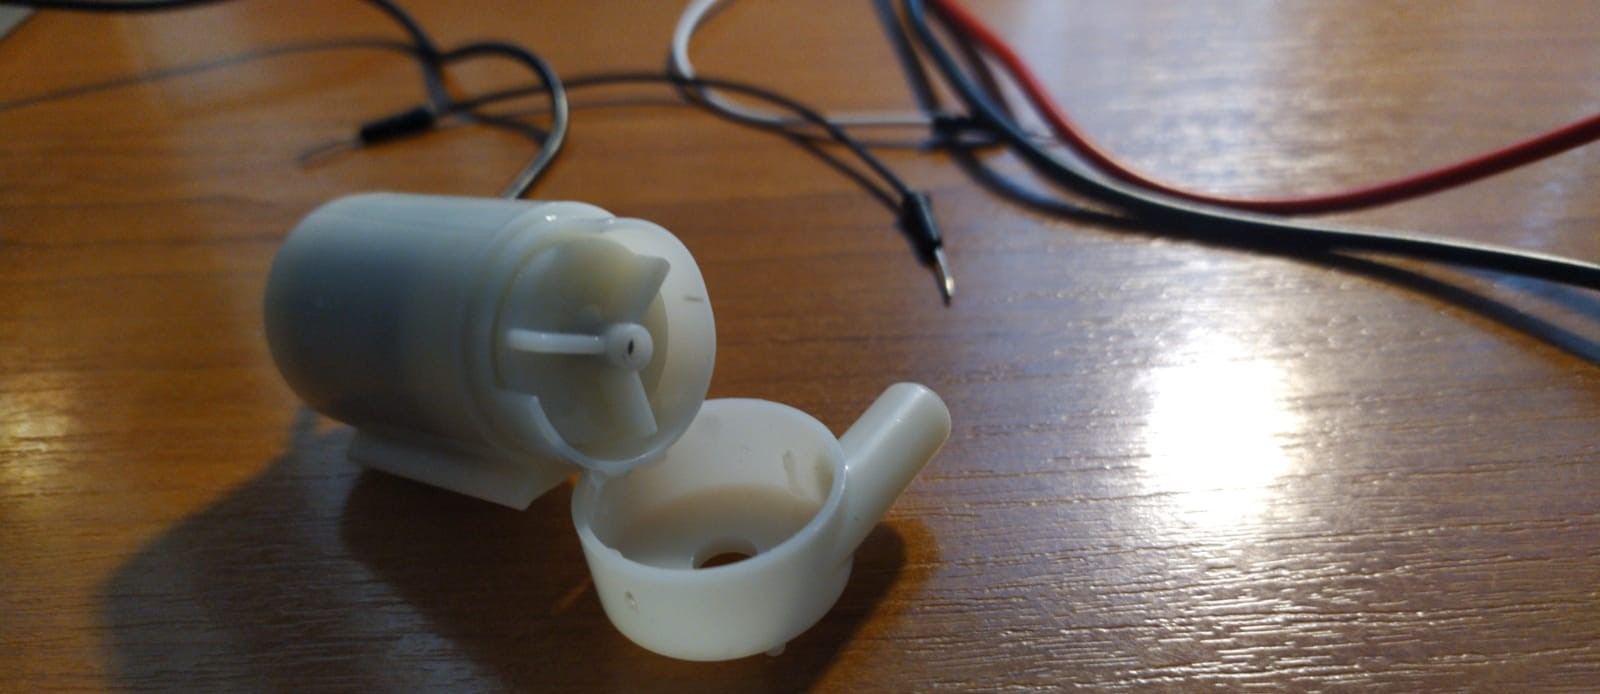
\includegraphics[width=\textwidth]{Pictures/pompa.jpeg}
\caption{Pompa de apa, se poate observa paleta rotativa si incaperea cu cele 2 orificii}
\end{figure}

Repararea pompei a reprezentat un proces prin care i s-a distrus integritatea fizica insa in cea mai mare masura aceasta a putut fi restaurata. Consumul pompei este de $\approx$ 300 mA, iar curentul maxim ce poate fi furnizat de unul dintre pinii generali ai microcontrolerului este de 40 mA, ceea ce inseamna ca nu va fi posibila comanda actuatorului direct de catre microcontroler. In acest caz solutia aleasa de noi este comandarea pompei prin intermediul unui tranzistor ce va comuta intre saturatie ("deschis") si blocare ("inchis"). Pompa va fi amplasata astfel incat curentul consumat sa fie curentul de colector al tranzistorului.

\newpage

\begin{figure}[H]
\centering
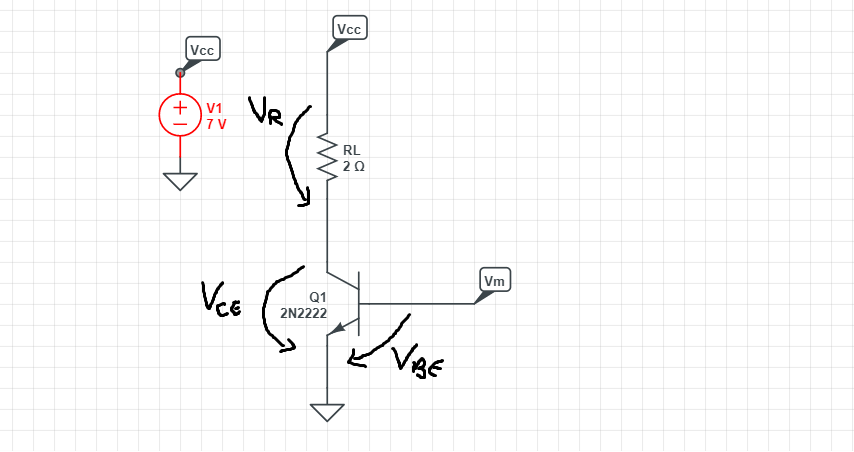
\includegraphics[width=\textwidth]{Pictures/tranz.png}
\caption{Schema prin care se doreste comandarea pompei de apa}
\end{figure}

Din cauza accesului limitat la piese, explicat in prima sectiune, am folosit cel mai adecvat tranzistor pe care l-am avut la dispozitie, acesta este tranzistorul bipolar NPN de tip 2N2222A. Pentru acest tranzistor am masurat un factor de amplificare static in curent $\beta \approx 300$. Vm reprezinta potentialul ce poate fi furnizat pe unul din pinii microcontrolerului, acesta avand la dispozitie pentru iesire numai pini digitali, deci Vm $\approx$ Vcc $\approx$ 5V. Tensiunea de functionare la care vom alimenta pompa este de 5V deci Vr trebuie sa fie minim 5V, pentru functionarea in saturatie s-a ales $V_{CE} \approx 2V$ ceea ce impune $V_{CC} \approx 7V$. \\
\begin{itemize}

\item $Vm = 0 \Rightarrow V_{BE} = 0; V_{CC} = 7V \Rightarrow V_{CE} > 0, V_{CB} > 0 \Rightarrow$ blocare. 

\item $Vm = 5V \Rightarrow V_{BE} > 0; V_{CC} = 7V \Rightarrow V_{CE} = 2V, V_{R} = 5V, V_{BC > 0} \Rightarrow$ saturatie.

\end{itemize}
In regim de saturatie transzistorul ar trebiu sa prezinte o rezistenta foarte mica colector-emitor pentru a permite curegerea celor 300 mA consumati de pompa. \newpage\textcolor{red}{ La implementarea practica a circuitului, la momentul aplicarii potentialului Vm, din motive pe care nu le cunoastem uC inceteaza sa functioneze, astfel circuitul nu a putut fi pus in practica. Avem ca solutie alternativa folosirea unui releu in locul tranzistorului}.

\section{Convertorul ADC}
\hspace{8 mm} Pentru a putea lua orice decizie sau pentru a putea calcula parametrii de interes este nevoie de cuantizarea marimilor citite de la senzori si transformarea acestora sub o forma ce poate fi prelucrata numeric. Microcontrolerul dispune de un convertor ADC ce poate face acesata transformare. Convertorul ADC lucreaza pe 10 biti si poate avea ca referinta de tensiune: pinul extern AREF (referinta interna dezactivata), pinul AVCC cu condendsator cuplat la pinul AREF catre masa, referinta interna de 1.1V sau referinta interna de 2.56V. In acest proiect am ales ca referinta de tensiune pinul AVCC. Tot ce presupune controlul convertorului se face cu ajutorul registrelor ADCSRA si ADCSRB. Pentru a activa convertorul trebuie setat bitul ADEN din registrul ADCSRA iar pentru a porni o conversie bitul ADSC din acelasi registru. In momentul finalizarii unei conversii, microcontrolerul seteaza bitul ADSC inapoi la 0 iar rezultatul conversiei este scris in registrul de 16 biti ADC format din registrele de 8 biti ADCL si ADCH. Cand ADCL este citit, registrul de date ADC nu este actualizat pana nu se citeste si ADCH.


\newpage

\section{ Schema electrica}
\begin{figure}[H]
\centering
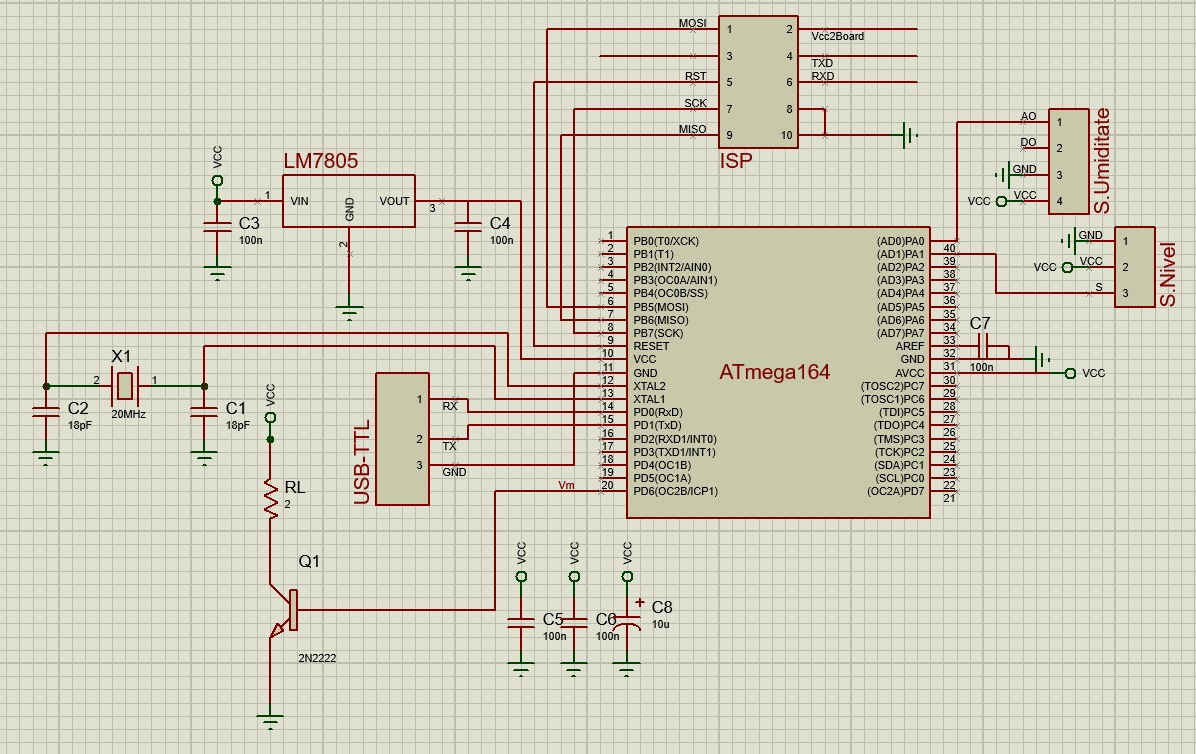
\includegraphics[width=\textwidth]{Pictures/schemael.jpeg}
\caption{Schema electrica a proiectului}
\end{figure}
\newpage

\section{ BOM (Bill of Materials)}


\begin{table}[H]
\begin{tabular}{|l|l|l|l|l|}
\hline
Clasa & Descriere & Distribuitor & Cantitate & Pret unitar  \\ \hline
Senzor & Senzor de nivel al apei & Optimus Digital & 1 & 3,29 Lei \\ \hline
Senzor & Senzor de umiditate a solului & Optimus Digital & 1 & 3,99 Lei \\ \hline
Actuator & Mini pompa de apa submersibila & Optimus Digital & 1 & 8,99 Lei\\ \hline
Programator & Programator USB ASP & Optimus Digital & 1 & 7,49 Lei\\ \hline
Stabilizator & Stabilizator de tensiune LM7805 & ETTI & 1 & - \\ \hline
Convertor & Convertor USB TTL & Optimus Digital & 1 & 12,89 Lei\\ \hline
Tranzistor & NPN 2N2222A & Optimus Digital & 1 & 0,99 Lei\\ \hline
Oscilator & Quartz, 20 MHz & ETTI & 1 & -\\ \hline
Condensator & Electrolitic, 1uF & Optimus Digital & 1 & 0,49 Lei\\ \hline
Condensator & Electrolitic, 10uF &Optimus Digital  & 1 & 0,49 Lei\\ \hline
Condensator & Ceramic, 22pF &Optimus Digital  & 2 & 0,49 Lei\\ \hline
Condensator & Ceramic, 100nF & Optimus Digital & 5 & 0,69 Lei\\ \hline
\end{tabular}
\end{table}

\newpage

\section{ Codul ce ruleaza pe microcontroler}

\begin{lstlisting}[style=CStyle]

#define F_CPU 20000000UL
#include <avr/io.h>
#include <util/delay.h>
#include <stdint.h>
#define MINUT 60000
#define VREF 5.1
#define DEBIT 0.43
#define BAUD 9600
#define MYUBRR F_CPU/16/BAUD-1

union {
	float f;
	char bytes[4];
} joinedFloat;

union {
	int i;
	char bytes[2];
} joinedInt;

float cantitateApa = -1; //L  // configurare numai prin aplicatie
int umiditatePrag = -1; //[%]  // configurare numai prin aplicatie  

void ADC_Init();
void USART_Transmit( unsigned char data );
void USART_Init( unsigned int baud );
unsigned char USART_Receive( void );
void Conversie(unsigned char *low, unsigned char *high);
void stateConnected(unsigned char command);
void stateReading(unsigned char command);
int preiaDateUmiditate();
int preiaDateNivel();

int main(void)
{
	//Initializare USART
	USART_Init ( MYUBRR );
	
	//Initializare ADC
	ADC_Init();

	//DDRD = 0xFF;
	unsigned char command;
	int umiditate; //[%]
	int nivel; // [mm]
	
    while (1) 
    {
		command = UDR0;
		if(command == 'c')
			stateConnected(command);
		umiditate = preiaDateUmiditate();
		if(umiditatePrag != -1)
			if(umiditate < umiditatePrag && cantitateApa != -1){
				nivel = preiaDateNivel();
				if(nivel > 0 && nivel <= 40){
					float t = cantitateApa / DEBIT; //Calcul timpul in care se tine pompa deschisa
					t *= 60; //Conversie in secunde
					const int timp = t * 1000; //Conversie in ms
					DDRD = 0xFF; //Setam portul D ca output
					PORTD = 0xFF; //Setam potentialul Vm la aprox. Vcc = 5V
					_delay_ms(1000); //Tinem pompa activa un anumit timp ------------------------> PROBLEMA
					PORTD = 0x00; //Inchidem pompa
					_delay_ms(MINUT);//Asteptam un minut pentru infiltrarea apei in sol
				}
			}	
    }
}

	//Returneaza umiditatea in procente
int preiaDateUmiditate(){
	
	//Selecteaza canalul ADC0 pentru conversie (XOR cu 0x01)
	ADMUX = ADMUX ^ 0x01;
	
	ADCSRA = (ADCSRA | (1 << ADSC)); //Porneste o conversie setand ADSC
	while((ADCSRA&(1<<ADIF))==0);   //Asteapta sa se termine conversia (ADSC resetat de hw)
	
	//A doua conversie deoarece din cauza schimbarii canalului
	//este posibil ca prima sa nu fie corecta
	//ADCSRA = (ADCSRA | (1 << ADSC)); //Porneste o conversie setand ADSC
	//while((ADCSRA&(1<<ADIF))==0);   //Asteapta sa se termine conversia (ADSC resetat de hw)
	
	unsigned int convLow = ADCL; //Citim ADCL
	unsigned int convHigh = (unsigned int)(ADCH << 8); //Citim ADCH si facem loc pentru ADCL shitand la stanga 8 pozitii
	unsigned int conv = convLow | convHigh; //Concatenam ADCL cu ADCH
	
	float resConv = (conv * VREF) / 1023.0; //Rezultatul conversiei in V
	int umiditate = -5 * (5*resConv -24); //Umiditatea in procente (0-100)
	
	return (umiditate / 10) * 10; //Discretizarea valorilor pe 10 intervale pentru a minimiza eroarea aprox. caracteristicii
	
}

	//Returneaza nivelul din vas in mm
int preiaDateNivel(){
	
	//Selecteaza canalul ADC1 pentru conversie (SAU cu 0x01)
	ADMUX = ADMUX ^ 0x01;
	
	ADCSRA = (ADCSRA | (1 << ADSC)); //Porneste o conversie setand ADSC
	while((ADCSRA&(1<<ADIF))==0);   //Asteapta sa se termine conversia (ADSC resetat de hw)
	
	//A doua conversie deoarece din cauza schimbarii canalului
	//este posibil ca prima sa nu fie corecta
	//ADCSRA = (ADCSRA | (1 << ADSC)); //Porneste o conversie setand ADSC
	//while((ADCSRA&(1<<ADIF))==0);   //Asteapta sa se termine conversia (ADSC resetat de hw)
	
	unsigned int convLow = ADCL; //Citim ADCL
	unsigned int convHigh = (unsigned int)(ADCH << 8); //Citim ADCH si facem loc pentru ADCL shitand la stanga 8 pozitii
	unsigned int conv = convLow | convHigh; //Concatenam ADCL cu ADCH
	
	float resConv = (conv * VREF) / 1023.0; //Rezultatul conversiei in V
	int nivel = (100 * resConv - 200) / 3; //Nivelul in mm (0-40)
	
	return nivel;
	
}

void stateConnected(unsigned char command){
	
	int OK = 0;
	
	while(command == 'c'){
		
		if(!OK){
			USART_Transmit('a'); //Transmitere mesaj de confirmare intrare in starea de conectat
			OK = 1;
		}
		int umiditate = preiaDateUmiditate(); //Se preia umiditatea
		int nivel = preiaDateNivel(); //Se preia nivelul apei
		unsigned char *p;
		p = (unsigned char*)&umiditate;
		USART_Transmit(*p++);
		USART_Transmit(*p);
		p = (unsigned char*)&nivel;
		USART_Transmit(*p++);
		USART_Transmit(*p);
		
		_delay_ms(2000);
		

		command = UDR0;
		if(command == 'r'){
			stateReading(command);
			command = UDR0;
			command = 'c';
		}
		else if(command != 'b')
			command = 'c';
			
	}
}

void stateReading(unsigned char command){
	
	int i;
	for(i=0;i<4;i++){
		joinedFloat.bytes[3-i] = USART_Receive();
	}
	
	cantitateApa = joinedFloat.f;
	
	for(i=0;i<2;i++){
		joinedInt.bytes[1-i] = USART_Receive();
	}
	
	umiditatePrag = joinedInt.i;
}


void ADC_Init()
{
	//Activeaza ADC, selecteaza intreruperile si
	//defineste frecventa de lucru a ADC la XTAL/2
	ADCSRA = 0x87;
	
	//Selecteaza Vref ca AVCC, rezultatul ajustat la dreapta
	//si canalul analog de intrare ca ADC0
	ADMUX = 0x40;
}

void USART_Init( unsigned int baud )
{
	/* Set baud rate */
	UBRR0H = (unsigned char)(baud>>8);
	UBRR0L = (unsigned char)baud;
	/* Enable receiver and transmitter */
	UCSR0B = (1<<RXEN0)|(1<<TXEN0);
	/* Set frame format: 8data, 2stop bit */
	UCSR0C = (1<<USBS0)|(3<<UCSZ00);
}

void USART_Transmit( unsigned char data )
{
	/* Wait for empty transmit buffer */
	while ( !( UCSR0A & (1<<UDRE0)) )
	;
	/* Put data into buffer, sends the data */
	UDR0 = data;
}

unsigned char USART_Receive( void )
{
	/* Wait for data to be received */
	while ( !(UCSR0A & (1<<RXC0)) )
	;
	/* Get and return received data from buffer */
	return UDR0;
}


\end{lstlisting}

\newpage

\section{ Codul aplicatiei de utilizator}


\begin{lstlisting}[style=CStyle]

using System;
using System.Collections.Generic;
using System.ComponentModel;
using System.Data;
using System.Drawing;
using System.Linq;
using System.Text;
using System.Threading.Tasks;
using System.Windows.Forms;

namespace P2
{
    public partial class Form1 : Form
    {
        bool isConnected = false;
        public Form1()
        {
            InitializeComponent();
            stateLabel.Text = "Neconectat";
            buttonDeconnect.Enabled = false;
            labelUmidVal.Text = "N/A";
            labelNivelVal.Text = "N/A";
            textBoxUmid.Text = "0";
            textBoxCantApa.Text = "0";
            textBoxUmid.Enabled = false;
            textBoxCantApa.Enabled = false;
            buttonSend.Enabled = false;
        }

        private void Form1_Load(object sender, EventArgs e)
        {
            comBox.Items.Add("COM1");
            comBox.Items.Add("COM2");
            comBox.Items.Add("COM3");
            comBox.Items.Add("COM4");
            comBox.Items.Add("COM5");
            comBox.SelectedIndex = 0;
            SerialPort.PortName = comBox.SelectedItem.ToString();
        }

        private void buttonConnect_Click(object sender, EventArgs e)
        {
            buttonConnect.Enabled = false;
            buttonDeconnect.Enabled = true;
            textBoxUmid.Enabled = true;
            textBoxCantApa.Enabled = true;
            buttonSend.Enabled = true;

            SerialPort.Open();
            SerialPort.WriteLine("c");
            char ack = (char)SerialPort.ReadChar();
            if(ack == 'a')
            {
                isConnected = true;
                    byte[] b = new byte[2];
                    b[0] = (byte)SerialPort.ReadByte();
                    b[1] = (byte)SerialPort.ReadByte();
                    int realtimevalue = b[1];
                    realtimevalue = realtimevalue << 8;
                    realtimevalue += b[0];
                    labelUmidVal.Text = realtimevalue.ToString() + " %";

                b[0] = (byte)SerialPort.ReadByte();
                    b[1] = (byte)SerialPort.ReadByte();
                    realtimevalue = b[1];
                    realtimevalue = realtimevalue << 8;
                    realtimevalue += b[0];
                labelNivelVal.Text = realtimevalue.ToString() + " mm";
            }
        }

        private void comBox_SelectedIndexChanged(object sender, EventArgs e)
        {
            SerialPort.PortName = comBox.SelectedItem.ToString();
        }

        private void buttonDeconnect_Click(object sender, EventArgs e)
        {
            SerialPort.WriteLine("b");
            buttonConnect.Enabled = true;
            buttonDeconnect.Enabled = false;
            textBoxUmid.Enabled = false;
            textBoxCantApa.Enabled = false;
            buttonSend.Enabled = false;
        }

        private void buttonUpdate_Click(object sender, EventArgs e)
        {
            buttonUpdate.Enabled = false;
            if (SerialPort.IsOpen && isConnected)
            {
                byte[] b = new byte[2];
                b[0] = (byte)SerialPort.ReadByte();
                b[1] = (byte)SerialPort.ReadByte();
                int realtimevalue = b[1];
                realtimevalue = realtimevalue << 8;
                realtimevalue += b[0];
                labelUmidVal.Text = realtimevalue.ToString() + " %";

                b[0] = (byte)SerialPort.ReadByte();
                b[1] = (byte)SerialPort.ReadByte();
                realtimevalue = b[1];
                realtimevalue = realtimevalue << 8;
                realtimevalue += b[0];
                labelNivelVal.Text = realtimevalue.ToString() + " mm";

            }
            buttonUpdate.Enabled = true;
        }

        private void buttonSend_Click(object sender, EventArgs e)
        {

            if(textBoxUmid.Text != "" && textBoxCantApa.Text != "")
            {
                float cantitateApa = float.Parse(textBoxCantApa.Text);
                SerialPort.WriteLine("r");
                isConnected = false;
                byte[] b = BitConverter.GetBytes(cantitateApa);
                SerialPort.WriteLine(b[0].ToString());
                SerialPort.WriteLine(b[1].ToString());
                SerialPort.WriteLine(b[2].ToString());
                SerialPort.WriteLine(b[3].ToString());

                int umiditatePrag = int.Parse(textBoxUmid.Text);
                byte[] bi = BitConverter.GetBytes(umiditatePrag);
                SerialPort.WriteLine(bi[0].ToString());
                SerialPort.WriteLine(bi[1].ToString());

                SerialPort.WriteLine("x");
                isConnected = true;
            }
        }

        private void Form1_FormClosed(object sender, FormClosedEventArgs e)
        {
            SerialPort.WriteLine("b");
            SerialPort.Close();
        }
    }
}

\end{lstlisting}
\newpage

\section{ Bibliografie}

\begin{itemize}

\item https://www.youtube.com/watch?v=IyGwvGzrqp8\& list=WL\& index=8\& t=0s

\item https://www.youtube.com/watch?v=F7NlCaaL3yU\& list=WL\& index=8\& t=0s

\item https://www.instructables.com/id/Serial-Port-Programming-With-NET/

\item https://www.edn.com/usart-vs-uart-know-the-difference/
\item https://www.allaboutcircuits.com/textbook/digital/chpt-3/logic-signal-voltage-levels/
\item https://www.edaphic.com.au/soil-water-compendium/soil-moisture-sensor-calibration/

\item https://electronics.stackexchange.com/questions/112441/using-a-transistor-as-a-switch
\item https://www.instructables.com/id/Avr-fuse-basics-Running-an-avr-with-an-external-cl/
\item https://www.engbedded.com/fusecalc/
\item https://app.diagrams.net/
\item https://www.avrfreaks.net/forum/converting-4-bytes-float-help

\end{itemize}
\end{document}